%%%%%%%%%%%%%%%%%%%%%%%%%%%%%%%%%%%%%%%%%
% Journal Article
% LaTeX Template
% Version 1.3 (9/9/13)
%
% This template has been downloaded from:
% http://www.LaTeXTemplates.com
%
% Original author:
% Frits Wenneker (http://www.howtotex.com)
%
% License:
% CC BY-NC-SA 3.0 (http://creativecommons.org/licenses/by-nc-sa/3.0/)
%
%%%%%%%%%%%%%%%%%%%%%%%%%%%%%%%%%%%%%%%%%

%----------------------------------------------------------------------------------------
%	PACKAGES AND OTHER DOCUMENT CONFIGURATIONS
%----------------------------------------------------------------------------------------

\documentclass[twoside]{article}

\usepackage[sc]{mathpazo} % Use the Palatino font
\usepackage{amsmath}
\usepackage[T1]{fontenc} % Use 8-bit encoding that has 256 glyphs
\linespread{1.05} % Line spacing - Palatino needs more space between lines
\usepackage{microtype} % Slightly tweak font spacing for aesthetics

\usepackage[hmarginratio=1:1,top=32mm,columnsep=20pt]{geometry} % Document margins
\usepackage{multicol} % Used for the two-column layout of the document
\usepackage[hang, small,labelfont=bf,up,textfont=it,up]{caption} % Custom captions under/above floats in tables or figures
\usepackage{booktabs} % Horizontal rules in tables
\usepackage{float} % Required for tables and figures in the multi-column environment - they need to be placed in specific locations with the [H] (e.g. \begin{table}[H])
\usepackage{tabularx}
\usepackage{hyperref} % For hyperlinks in the PDF
\usepackage{cleveref} % For clever referencing

\usepackage{lettrine} % The lettrine is the first enlarged letter at the beginning of the text
\usepackage{paralist} % Used for the compactitem environment which makes bullet points with less space between them

\usepackage{abstract} % Allows abstract customization
\renewcommand{\abstractnamefont}{\normalfont\bfseries} % Set the "Abstract" text to bold
\renewcommand{\abstracttextfont}{\normalfont\small\itshape} % Set the abstract itself to small italic text

\usepackage{titlesec} % Allows customization of titles
%\renewcommand\thesection{\Roman{section}} % Roman numerals for the sections
%\renewcommand\thesubsection{\Roman{subsection}} % Roman numerals for subsections
\titleformat*{\section}{\large\centering\bfseries} % Change the look of the section titles
\titleformat*{\subsection}{\large\bfseries} % Change the look of the section titles

\usepackage{fancyhdr} % Headers and footers
\pagestyle{fancy} % All pages have headers and footers
\fancyhead{} % Blank out the default header
\fancyfoot{} % Blank out the default footer
\fancyhead[C]{Running title $\bullet$ November 2012 $\bullet$ Vol. XXI, No. 1} % Custom header text
\fancyfoot[RO,LE]{\thepage} % Custom footer text
\usepackage[Table]{xcolor}
\usepackage{todonotes}
\usepackage{menukeys}
\usepackage[utf8]{inputenc}
\usepackage{pgfplots}
\usepackage{natbib}
\pgfplotsset{compat=1.9}%compatability for tikz functionality
\def\citeapos#1{\citeauthor{#1}'s (\citeyear{#1})}

%----------------------------------------------------------------------------------------
%	TITLE SECTION
%----------------------------------------------------------------------------------------

\title{\vspace{-15mm}\fontsize{24pt}{10pt}\selectfont\textbf{Automatic optimization of parameters for Ocular Artifact Correction in EEG}} % Article title

\author{
\large
\textsc{Benjamin Ahm, } % Your name
\textsc{Emil Riis Hansen, }
\textsc{Kristian Hauge Jensen, }\\
\textsc{Morten Korsholm Terndrup}\\[2mm]\thanks{A thank you or further information}
\normalsize Aalborg University \\ % Your institution
\normalsize \href{mailto:mternd13@student.aau.dk}{mternd13@student.aau.dk} % Your email address
\vspace{-5mm}
}
\date{}

%----------------------------------------------------------------------------------------

\begin{document}

\maketitle % Insert title

\thispagestyle{fancy} % All pages have headers and footers

%----------------------------------------------------------------------------------------
%	ABSTRACT
%----------------------------------------------------------------------------------------

\begin{abstract}

\noindent Brain-Computer Interfaces (BCI) is becoming increasingly useful for things such as diagnosing brain conditions and restoring motor function in disabled people. One area that still needs to improve is artifact correction. In this study, a state-of-the-art artifact correction method dubbed OACL is expanded upon in order to make it more generally applicable. The new method (MCOACL) is a multi-class version of OACL that does not require expert input. We use Filter Bank Common Spatial Pattern (FBCSP) for feature extraction, followed by Random Forest (RF) for classification. To evaluate the method it is put in a pipeline A consisting of MCOACL $\to$ FBCSP $\to$ RF, which is then compared to an identical pipeline B without MCOACL. The hyperparameters for these pipelines are optimized using Bayesian Optimization (BO). The 4-class EEG data from dataset 2a of BCI Competition IV, comprising 22 EEG channels and 2 sessions of 9 subjects over 6 runs, is used to evaluate the method. The results from pipeline A did not yield better classification results than pipeline B. The result might however stem from parameters  not being optimized correctly.

\end{abstract}

%----------------------------------------------------------------------------------------
%	ARTICLE CONTENTS
%----------------------------------------------------------------------------------------

\begin{multicols}{2} % Two-column layout throughout the main article text


\section{Introduction}\label{sec:introduction}
% Relevance. What is the general motivation ---> What is the concrete problem.
The field of Brain-Computer Interfaces (BCI) has in recent years been under active research, especially with the popularity of machine learning techniques. The reason for the interest is the many useful application of a well-working BCI, such as replacing lost motor function in disabled people, helping with analysis in brain imaging to diagnose brain conditions or novel applications in computer games. 

The general idea of a BCI is to measure brain activity usually represented by electroencephalogram (EEG) signals, by putting sensors on the scalp that can measure the electric impulses. Each sensor is referred to as a channel in the EEG data. However, the EEG data is noisy at best, and this problem can severely affect the results of classification algorithms. Furthermore, EEG data can consist of hundreds or even thousands of samples per second, depending on the sensory equipment, which makes the dimensionality of EEG data too large for many classification algorithms. Therefore, artifact removal and feature extraction are important steps in any given BCI.

\cite{uriguen2015eeg} argues that non-physiological artifacts can usually be avoided or trivially removed. The physiological artifacts they have found to be most common are electrooculographic (EOG), electromyographic (EMG), and electrocardiographic (ECG) signals. They are also referred to as ocular, muscle, and cardiac artifacts respectively. Additionally, artifact removal can be done with or without a reference signal such as the EOG, and semi-automatically or automatically (that is, with or without human intervention). Methods that do not need reference signals are more generally applicable, since reference signals are not always recorded and may be preferable not to measure for the comfort of the subjects. Additionally, methods that are automatic are preferred to semi-automatic ones, since the interaction required in the latter usually necessitates the opinion of an expert.

%2. Explain the problem that you study — be clear, do not dive into unnecessary details.
This leaves us with the problem of deciding which techniques should be applied to obtain a corrected EEG signal, and consequently an accurate model that classifies the EEG data. Each technique may require several hyperparameters that need tuning to achieve the optimal results, such as regularization parameters in machine learning algorithms. Such tuning is usually done manually, by experimenting with different values to see their effect on some validation data. Users of the BCI or medical professionals might be knowledgeable about tuning some of the parameters but not all, hence it requires either an expert to help determine them or extensive personnel training. Nonetheless, it often requires a great deal of time tuning the parameters to obtain satisfactory results. Another, more useful approach, would be to automatically infer the hyperparameters from the training data. Such automatic parameter tuning has had positive results through Bayesian optimization \citep{brochu2010tutorial,snoek2012practical,shahriari2016taking} which is an optimization technique that minimizes an unknown objective function by building a Bayesian probabilistic model of the function. The probabilistic model is built by treating the objective function as a black box.

%3  Describe your achievements — you can for example list them.
We propose a technique for correcting artifacts from EEG data based on the method by \citep{li2015ocular}. We adapt the technique for use in multi-class datasets by optimizing hyper-parameters for the artifact correction through Bayesian optimization. This is different from the original approach, where parameters were either manually set or determined by binary logistic regression.

%5 Give an overview of the sections to follow
The paper is structured as follows. In \cref{sec:relatedwork} we consider related work. In \cref{sec:oacl} we explain the artifact correction scheme and how our adaptation differs from the original technique (OACL) proposed by \citet{li2015ocular}. In \cref{sec:feature-extraction} we discuss how to extract features from the corrected EEG time series by applying the Filter Bank Common Spatial Patterns algorithm. In \cref{sec:randomforest} we discuss classification of EEG features by the Random Forest classification algorithm. We then explain how we apply Bayesian optimization to optimize hyperparameters in \cref{sec:bayesian-optimization}. Finally, we evaluate and discuss the results in \cref{sec:results}.

%4  Comment on related work — compare your approach with others; mention both the strengths and weaknesses.
\subsection{Related Work} \label{sec:relatedwork}
% Artifact Removal
Many methods exist for artifact correction in EEG signals. Well-known ones such as \emph{Principal Component Analysis} (PCA), \emph{Independent Component Analysis} (ICA), and \emph{Wavelet Transform} (WT) have shown various results in the research area regarding their effect on the classification of EEG data   \citep{uriguen2015eeg}. Both PCA and ICA are examples of \emph{Blind Source Separation} techniques. PCA is used to reduce the dimensionality of the data, and will return the principal components that maximize the variance of the data. ICA is a way of computing the independent components of a linear combined mixed source. WT can be used to decompose a signal into components describing the frequency over time of a signal. \cite{krishnaveni2006automatic} have used WT to automatically detect and remove ocular artifacts, but the efficiency of their method remains to be tested.

Other approaches such as \emph{Eye Movement Correction Procedure} (EMCP) \citep{gratton1983new} utilize EOG signals measured from the eyes of the subject to detect ocular artifacts and then estimate a propagation factor that can be used to determine the amount of EOG to remove from the EEG signals. \cite{hoffmann2008correction} later did a review of EMCP and ICA, and found that even though these methods reduced the mutual information between the EOG and EEG signals, there were still residual artifacts present up to 250 ms afterwards. \cite{li2015ocular} have had positive results in estimating a pseudo-EOG signal for binary class EEG data, making it possible to obtain an artifact signal without using a reference signal. Key benefit of this approach is that artifacts can be corrected from EEG signals alone, which obviates the difficulty of handling the mutual effects between EEG and EOG signals.

% Feature extraction
The EEG measured on a channel forms a time series where the changes in amplitude over time contain the information that is to be classified. In order to reason about the data, this information must be extracted into features that can be used to train a classifier. Application of ICA, PCA, or WT directly extracts components that can be used as feature vectors \citep{uriguen2015eeg}. Another related technique is the \emph{Common Spatial Patterns} algorithm (CSP). CSP has been successful in extracting features that maximize the potential for classification in EEG data \citep{ang2008filter,ang2012filter}.

% Classification of EEG
For classification of EEG feature vectors, several algorithms have been successful in achieving good results. The survey by \citet{chan2015systematic} on the performance of ensemble methods in EEG contexts argues that the classification algorithm Random Forests more accurately classifies EEG data than other well-known methods such as k nearest neighbors and Support Vector Machines. \citet{sun2007experimental} also surveys the effectiveness of ensemble methods, but argues that performance is subject to the choice of base classifier as weak learners. 

% Automatic parameter tuning
Several methods for (automatic) hyperparameter optimization exist such as grid search, random search, Bayesian optimization, and gradient-based hyperparameter optimization. Grid search is the most straightforward of the methods, but also the slowest since the approach is to evaluate all combinations of the parameters. Random search does not need to exhaustively try all combinations in the search space, but starts at a random position in the search space and then evaluates new positions until some termination criterion is met. Bayesian optimization uses Gaussian processes to model an objective function with evaluations of the objective function as the posterior. The usefulness of Bayesian optimization is that it is possible to optimize over non-differentiable objective functions, since the objective function is treated as a black box. Gradient-based hyperparameter optimization uses reverse-mode differentiation in order to estimate the gradient of function, which can then be optimized using gradient descent.
% Someone proposed to make several passes over eeg to remove a single type of artifact?


%\subsection{Overview}
%Ocular artifacts such as eye movements or blinking are often present in EEG data, and can be the cause for significant decrease in classification accuracy. The reason for this, is that the amplitude of a signal changes when eye movements happen and can introduce uncertainty about the information hidden in the signal that we are interested in classifying. In order to reduce the impact of these ocular artifacts, we use the OACL technique proposed by \citet{li2015ocular} and generalize it to handle multi-class EEG data. Additionally, we optimize the hyperparameters with Bayesian Optimization (BO). Our approach is illustrated in \cref{fig:ProgramPipeline}. The preprocessing steps consist of correcting artifacts from the data using OACL, then the corrected data is bandpass filtered to create a filterbank, each of the filters is then spatially filtered using CSP with a one-versus-rest approach, and then the spatially filtered data for each sub-band is classified.


%------------------------------------------------

\section{Optimization of parameters for Ocular Artifact Correction}
short overview, maybe show a figure describing the pipeline.
\begin{figure*}%[!hbtp]
	\centering
	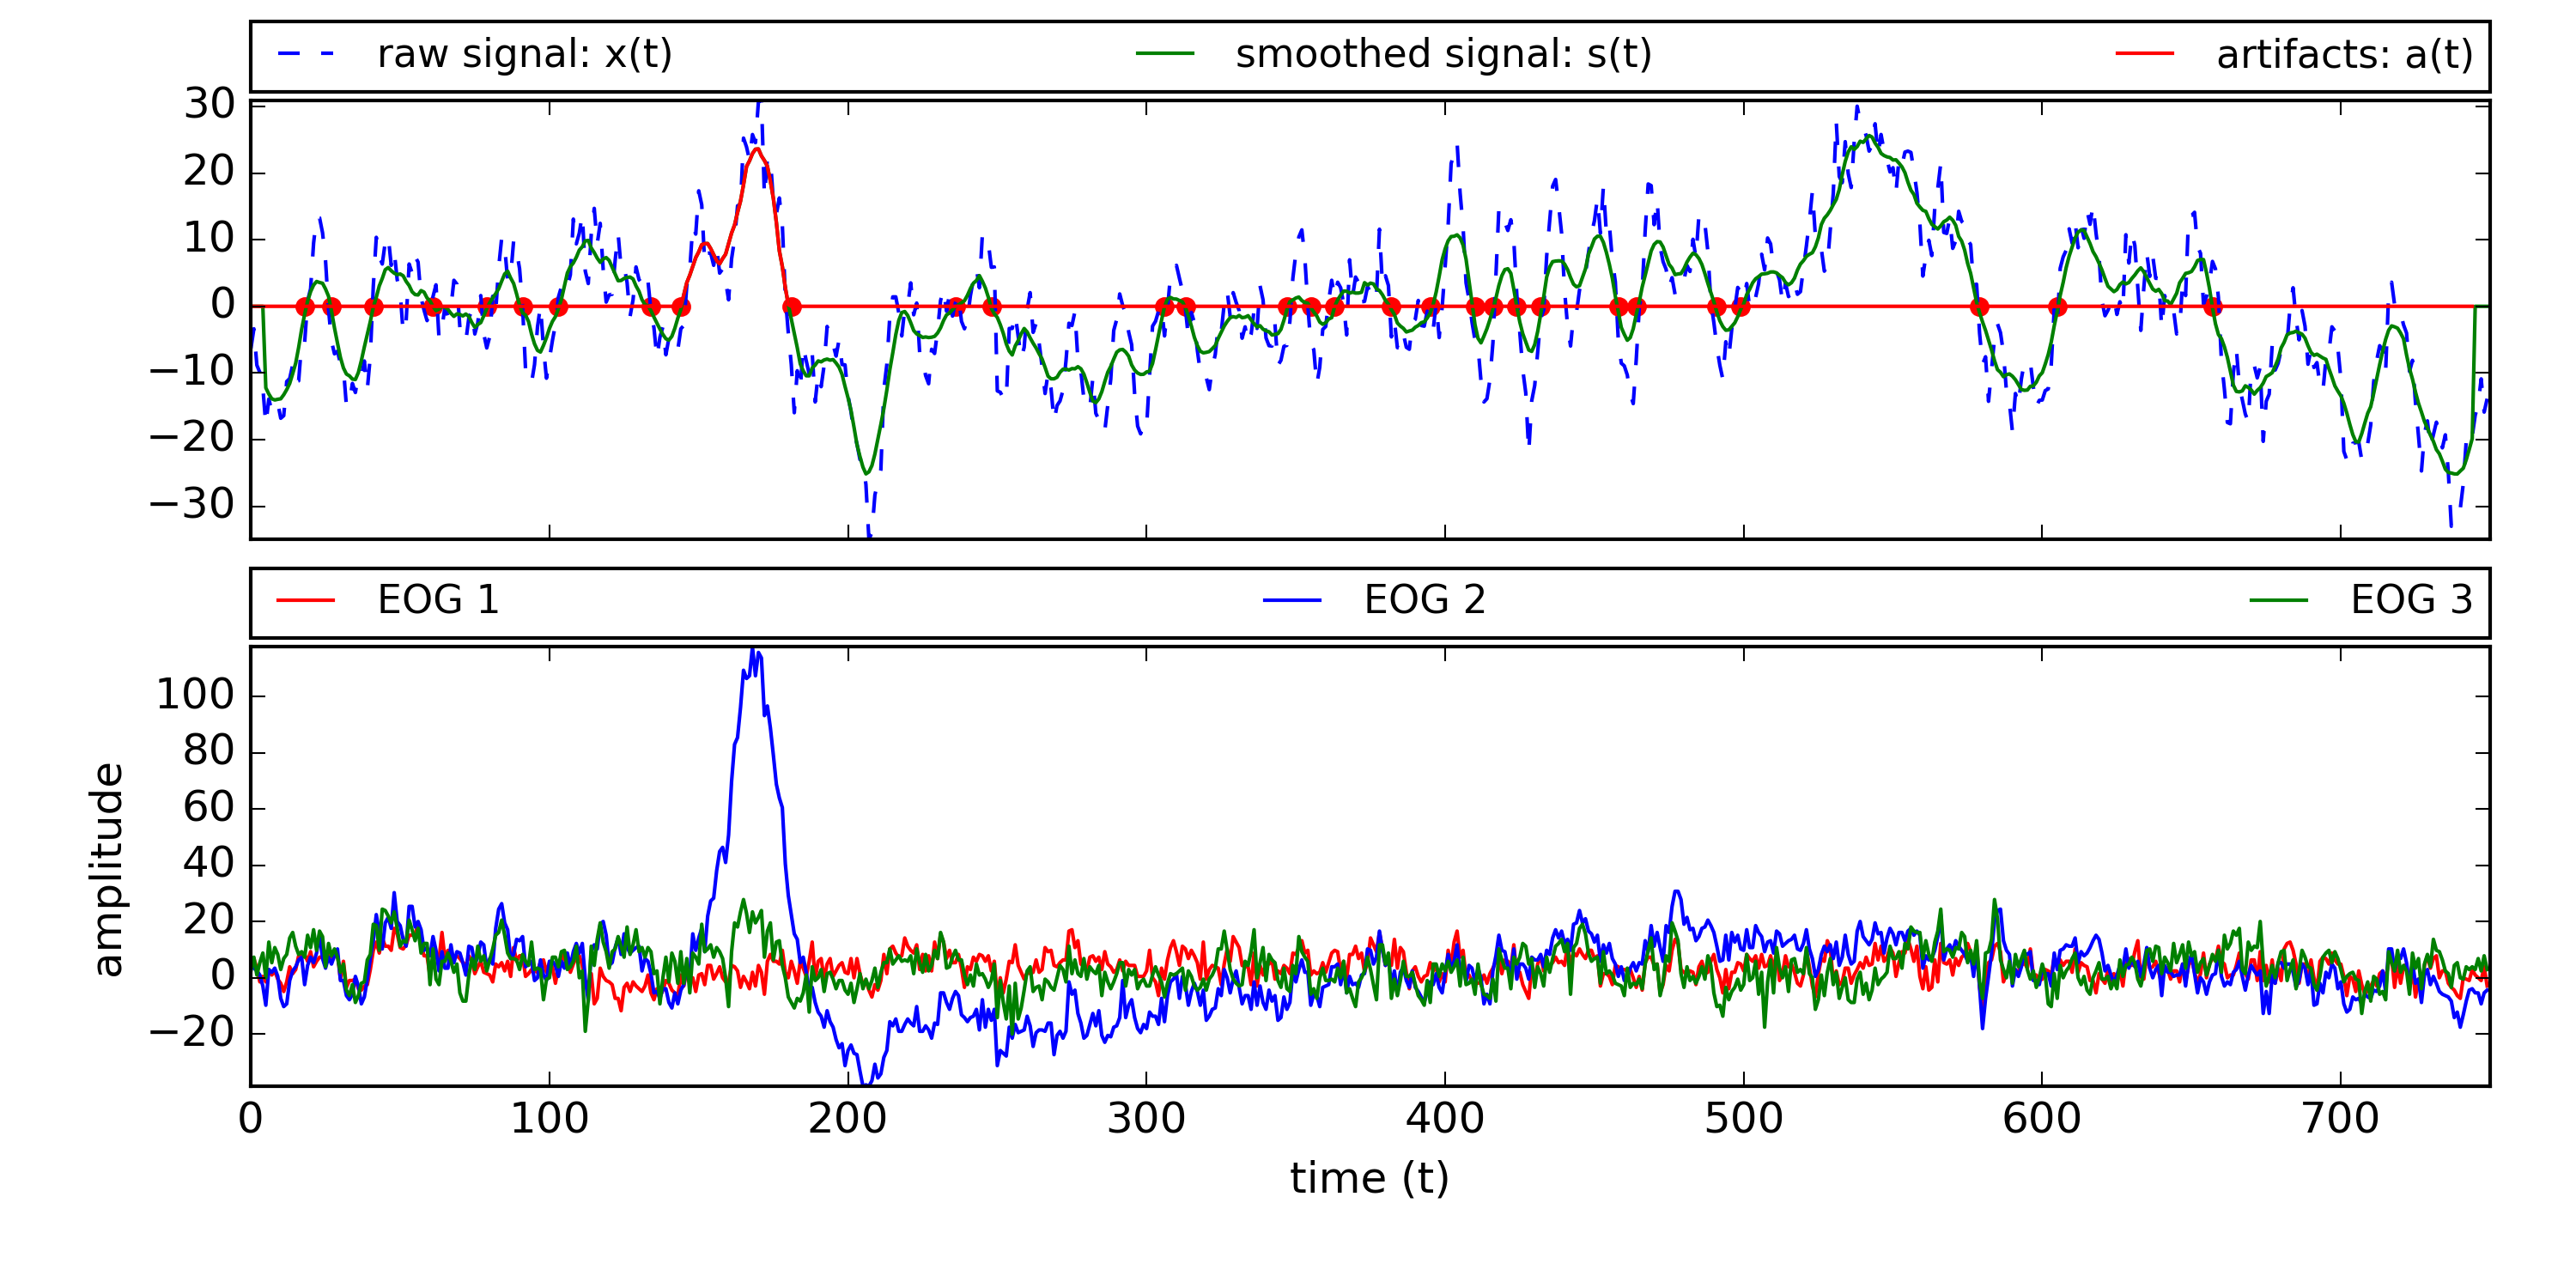
\includegraphics[width=1\textwidth]{figures/oacl-signals.png}
	\vspace{-2em}
	\caption{Smoothed signal and artifact signal superimposed on the raw EEG signal for a single channel in part of a single trial. The 3 EOG signals show ocular artifacts. The red artifact signal shows correct detection of artifact in this trial.}
	\label{fig:oacl-signals}
\end{figure*}
\section{Ocular Artifact Correction}\label{sec:oacl}
The OACL method consists of two parts: artifact detection and artifact removal. First, the raw EEG signals are processed to obtain the artifact signals, representing the parts of the signal that are artifacts. Then we find the \emph{filtering parameter} $\theta$ for each of the artifact signals, which determines the amount of each signal that needs to be removed from the raw signal in order to obtain the corrected signal. 
Since the original OACL method \citep{li2015ocular} was devised for binary class datasets, we generalize the algorithm for multi-class datasets. 

An EEG signal is an ordered collection of $n$ samples. Let $x = (s_0,...,s_t,...,s_n)$ where $s_t \in \mathbb{R}$ denotes the EEG sample for a channel. For simplicity, we can interpret $x$ as a function $x : \mathbb{N}_{\geq 0} \rightarrow \mathbb{R}$ where $x(t)$ denotes the amplitude of $x$ at time $t$. 
From $x(t)$ we perform all steps in artifact detection and removal.

%Let $t \in \mathbb{N}_{\geq 0}$ be the time of a EEG sample, then $x(t)$ denotes the amplitude measured at time $t$, that is, $x(t)$ denotes the raw EEG signal for some channel.

\subsection{Artifact Detection}
The goal of artifact detection is to find an artifact signal $a(t)$ from $x(t)$ that represents the parts of $x(t)$ that contain ocular artifacts. Before finding the artifact signal $a(t)$, we first obtain a smoothed signal by applying a \emph{moving average filter} to $x(t)$, in order to smooth out short-term fluctuations e.g. from external interference. A moving average filter is a function $s: \mathbb{N} \rightarrow \mathbb{R}$ that given time t, computes the average of $\frac{m}{2}$ samples on either side of the t\textsuperscript{th} sample. 

\begin{equation}
\label{eq:movavg}
s(t) = \frac{1}{m}\sum_{t-\frac{m}{2}}^{t+\frac{m}{2}}x(t)
\end{equation}
where $m$ is an odd number of neighboring points used to smooth the signal. The raw signal $x(t)$ and the corresponding smoothed signal $s(t)$ are illustrated in \cref{fig:oacl-signals}. 

From the smoothed signal $s(t)$ the OACL method finds the changes in amplitude between the samples, which could indicate eye movement. Therefore, we proceed by computing the relative heights between samples as the maximal difference in amplitude between a sample at time $t$ and its neighboring samples.

\begin{align*}
\Delta (t) = max(&|s(t)-s(t-1)|,\\
&|s(t+1) - s(t)|) \numberthis \label{eq:relheights}
\end{align*}
where we can consider $\Delta(t)$ as describing the fluctuations in the signal.

Now, we want to have some measure of what an artifact signal looks like. \citet{li2015ocular} found by inspection that ocular artifacts generally occur with sudden changes in amplitude ($\Delta$) measured in $\mu V$ in the intervals $]30; 70[$ and $]70; 150[$. The problem with this approach is, that it does not generalize to data collected using different setups for the EEG measurement. For this reason, we automatically estimate the ranges by considering them parameters to be optimized through Bayesian Optimization, discussed in \cref{sec:bayesian-optimization}.
For now, assume that we have some range $r \in R$ where
\begin{equation}\label{eq:ranges}
R=\{(l, u) \ | \ l,u \in \mathbb{N}_{\geq 0} \text{ and } l \leq u \}
\end{equation}
Note that we can have an arbitrary number of ranges; one for each artifact characteristic. For brevity, assume we have a single range r.

Now we can find the sample indexes $t$ where $\Delta (t)$  lies in the range $r$:
\begin{align*}
P = \{t \ | \ &\frac{m}{2} < t < n-\frac{m}{2}  \quad \textnormal{and} \\
& l < \Delta (t) < u\} \numberthis \label{eq:peaks}
\end{align*}
where $n$ is the number of samples in $x(t)$, and $P$ contains the indexes of samples in $s(t)$ where a change in amplitude lies within the range that characterizes an ocular artifact.

We now have the peaks of the ocular artifacts in $s(t)$, but we still need all of the artifact before we can correct it. The approach in the OACL method is to define the artifact to be from the closest zero point before the peak, to the closest zero point after the peak. We can now find the artifact signal as
\begin{equation}\label{eq:artifactsignal}
a(t) =
\begin{cases}
s(t)      & \quad \text{if } z_b \leq t < z_a\\
0  & \quad \text{otherwise}\\
\end{cases}
\end{equation}
where $z_b, z_a$ are the zero points before and after respectively. The concept of zero points of an artifact are illustrated in \cref{fig:oacl-signals}, where zero points can be seen as red dots. 

Zero points are found from the smoothed signal, by iterating through P, finding zero-crossings from sample to sample. 
Let again $s(t)$ be the function for the smoothed signal defined in \cref{eq:movavg}. We now iterate through all values of $t$, where $t \in P$, finding $Z \subset P$ as 
\begin{align*}
Z = \{t \ | \ s(t) \leq 0 \Rightarrow &(s(t+1) > 0 \ \vee \\
& s(t-1) > 0)\}
\numberthis\label{eq:zero_points}
\end{align*}
$Z$ will then be a list of indexes $\{z_1,...z_m\}$, that is used as the zero points $z_b$ and $z_a$ in \cref{eq:artifactsignal}. We can then find the correct zero points for a given peak, by finding predecessor and successor indexes in $Z$ for the index of a given peak in the artifact signal.

Recalling that we can use an arbitrary number of ranges in \cref{eq:ranges}, we obtain the set of artifact signals for a single channel of a single trial as:
\begin{equation}\label{eq:artifact-signals}
A(t)=  \begin{pmatrix}
a_1(t) \\
a_2(t) \\
\vdots  \\
a_l(t) 
\end{pmatrix}
\end{equation}
where $a_i(t)$ is the artifact signal found with the ith range and $l$ is the number of ranges.
The idea behind this, is that different types of artifacts can be found by using different ranges. 
\subsection{Artifact Removal}
With the artifact signals $A(t)$ extracted from the raw EEG data the next task is to remove the artifacts characterized by $A(t)$ from the original signal $x(t)$. Since signals are closed under subtraction we can obtain the corrected signal $c(t)$ by subtracting artifact signal from the EEG signal as
\begin{equation}\label{eq:corrected-signal}
c(t) = x(t) - \theta^T A(t)
\end{equation}
where $\theta \in \mathbb{R}^{k}$ is the \emph{filtering parameter}. $\theta$ is a vector with the factors determining the percentage of the artifact signal to subtract from the raw signal. 

The original approach of OACL is to obtain the $\theta$ parameter by training a binary logistic regression classifier with a modified hypothesis function. In this hypothesis function, the latent variable is derived from the power of the raw signal. Instead, we consider $\theta$ parameters as hyperparameters to the ocular artifact detection, which means that we can find the values for $\theta$ by optimizing them through the Bayesian optimization algorithm. In short, this means that we find the corrected signals for one subject as
\begin{align}\label{eq:corrected-signal}
C(t)=  \begin{pmatrix}
c_1(t) \\
\vdots  \\
c_{k}(t) 
\end{pmatrix}
\end{align}
where $k$ is the number of channels. By \cref{eq:corrected-signal} this means that the number of $\theta$ parameters we optimize over is $k \times l$, where $l$ is the number of artifact signals in \cref{eq:artifact-signals}. As we expect to remove 0-100\% of the artifact signal from the raw signal, we constrain $\theta \in \mathbb{R}^{l\times n}_{[0,1]}$.


\section{Feature Extraction}\label{sec:feature-extraction}
% Repeat why feature extraction
% What and why CSP
As mentioned in \cref{sec:introduction} raw EEG data consists of time series of amplitude samples. In such datasets, the information relevant for classification is hidden within the progression of the signal over time, and therefore it is not useful to consider each sample in the time series as a feature. For this reason we must perform feature extraction to extract the information relevant for classification. 

To extract the EEG features we use the \emph{Common Spatial Patterns} algorithm (CSP), which produces spatial filters that project the EEG data onto the subspace that best discriminates the classes.
CSP has been shown to perform well under the assumption that there is information relevant for classes hidden in the variances between the time series, which is the case in EEG data \cite{ang2012filter}. CSP is discussed in \cref{sec:csp}

% What and Why Filter bank
Moreover, \cite{ang2012filter} discusses that some frequencies are more relevant than others in EEG classification, and that the relevant frequencies vary between subjects. A way to find the informative frequencies is to use a bandpass filter to remove the frequencies above and below some threshold values, and leave us with a frequency band in between the threshold values. These are then used in our multi-class variant of FBCSP (a \emph{Filter Bank} (FB) combined with CSP) as proposed by \citet{ang2012filter}. Filter banks are described in \cref{sec:filterbank}.

\subsection{Common Spatial Patterns}\label{sec:csp}
%We have chosen to use a Filter bank multi class common spatial patterns (FBMCCSP) algorithm, for the purpose of extracting features from EEG data. The CSP algorithm has been used in several EEG classification studies within recent years, as in \cite{ang2012filter}. In all studies,\todo{source?} CSP were considered a step of improvement to the classification of EEG classes. Based on these results, we chose to incorporate CSP as part of the classification pipeline. 
The Common Spatial Patterns algorithm finds spatial filters that, when applied to signals, give the maximal mutual information between these with respect to signal variance. The method assumes there are classification information hidden within the variance between signals. Since we are classifying on motor imagery for different body parts, this assumption can be justified \citep{blankertz2008optimizing}.

Formally, CSP combines data with the same class. Let $\pmb{A}$ and $\pmb{B}$ be matrices of combined trials for class 1 and 2 respectively,

\begin{equation}
\label{eq:csp_data}
\pmb{A}, \mathbf{B} \in \mathbb{R}^{k*n}
\end{equation}
where $k$ and $n$ are the number of channels (signals) and samples respectively. CSP now calculates the covariance matrices for $\pmb{A}$ and $\pmb{B}$,

\begin{equation}
\label{eq:covariance_matrice}
\pmb{A_{cov}} = \frac{(\pmb{A} \cdot \overline{\pmb{A}})^\mathsf{T}  \cdot (\pmb{A} \cdot \overline{\pmb{A}})}{n - 1}
\end{equation}
where elements of $\overline{\pmb{A}}$ is defined as,

\begin{equation}
\label{eq:a_bar}
\pmb{\overline{A}_{ij}} = \frac{\pmb{A_{i,1}} + \pmb{A_{i,2}} + ... + \pmb{A_{i,n}}}{n}
\end{equation}

By applying simultaneous diagonalization between $\pmb{A_{cov}}$ and $\pmb{B_{cov}}$, we form the eigenvectors as the columns of $\pmb{P}$. $\pmb{P}$ is found when both of the following diagonalizations hold, 
\begin{equation}
\label{eq:diagonalization_A}
\pmb{P} \cdot \pmb{A_{cov}} \cdot \pmb{P^{-1}} = \pmb{D}, \quad \pmb{P}, \pmb{D}, \pmb{A_{cov}} \in \mathbb{R}^{k \times k}
\end{equation}
where D is a diagonal matrix consisting of the eigenvalues for $A_{cov}$, and
\begin{equation}
\label{eq:diagonalization_B}
\pmb{P} \cdot \pmb{B_{cov}} \cdot \pmb{P^{-1}} = \pmb{I}, \quad \pmb{P}, \pmb{I}, \pmb{B_{cov}} \in \mathbb{R}^{k \times k}
\end{equation}
where $\pmb{I}$ is the identity matrix. The spatial filter will now correspond to the first column of $\pmb{P}$, such that $\pmb{\vec{w}} = \pmb{P}^\mathsf{T}_{1}$ 

$\pmb{\vec{w}}$ can now be used as a linear transformation which, when applied to EEG signals, maps these into a new space, where signal features are more discriminative. The drawback of CSP is that it does not work well if the frequency bands are not adjusted to fit each subject \citep{novi2007sub}.

Generally, CSP only works for binary classes, whereas many real world applications require a greater number of classes. As our dataset has 4 classes, we use the one-vs-rest approach as proposed by \cite{ang2012filter} to extend CSP to multi-class. The one-vs-rest (OVR) method constructs one CSP per class, by choosing a class, and considering every other class as being the same. In this way, we obtain 4 binary CSPs, each constructed to create the maximum variance to all other classes. Step 7 in \cref{fig:ProgramPipeline} depicts the creation of four CSPs (one for each class versus the rest) in each sub-band for a total of 12 CSPs. Features can now be extracted by applying the spatial filters from CSP to EEG trials.

Our approach is to apply each CSP to every trial, and combine all of their respective feature vectors. As an example, say we have $m$ CSP, after applying OVR over all classes, for all bands. If now we apply one of the $m$ CSP to a single trial, we get a feature vector with $h$ components. The number of components is a parameter to the CSP algorithm that we optimize with Bayesian optimization.

By applying all CSPs to the same trial, and combining the resulting feature vectors, we get a trial with $h * m$ features. We apply this method on all trials in the dataset, from which $h * m$ features are found for every trial. These features are then used as the training set for a classifier.

For the implementation of CSP, we use the mne-toolbox by \citep{gramfort2014mne} library for Python.
\begin {figure*}%[!hbtp]
\centering
\begin{adjustbox}{width=\textwidth}
\begin{tikzpicture}

% Variables
\pgfmathsetmacro{\bs}{0.5};
\pgfmathsetmacro{\boxl}{2};
\pgfmathsetmacro{\boxh}{1};
\pgfmathsetmacro{\ll}{1};
\coordinate (blength) at (0.5, 0);
\coordinate (linel) at (1, 0);
\coordinate (bh) at (0, 1);
\coordinate (bl) at (2, 0);
\newcommand*{\fblist}{-3, 0, 3}
\newcommand*{\csplist}{-2, -1, 0, 1}

% Coordinate for start circle
\coordinate (trains) at (0, 0);

% Coordinate for Bayesian Optimization
\coordinate (bos) at ($(trains) + (blength) + 3/2*(linel)$);

% Coordinate for cross validation
\coordinate (crosss) at ($(bos) + (blength) + 3/2*(linel) + 1/2*(bl)$);

% Coordinate for Ocular Articaft Correction
\coordinate (oacls) at ($(crosss) + (bl) + (linel)$);

% Coordinate for Filter Bank
\coordinate (filters) at ($(oacls) + (bl) + (linel)$);

% Coordinate for filterbank nodes
\coordinate (filterbanks) at ($(filters) + 1/2*(bl) + 1.5*(linel) + 1/2*(blength)$);

% Coordinate for csp ovr nodes
\coordinate (cspovrs) at ($(filterbanks) + 1/2*(blength) + (linel)$);

% Coordinate for Random Forest Learner nodes
\coordinate (randomforestlearner) at ($(cspovrs) + 1/2*(blength) + 3.5*(linel)$);

% Coordinate for result node
\coordinate (results) at ($(randomforestlearner) + 1/2*(bl) + 1/2*(blength) + (linel)$);

% Coordinate for mean results
\coordinate (meanresults) at ($(results) + (blength) + (linel)$);

% Cooordinates for start and end of step box
\coordinate (boxceil) at (0, 6);
\coordinate (boxfloor) at (0, -6);
\coordinate (startbox) at ($(trains) + (-1, 0)$);
\coordinate (endbox) at ($(meanresults) + (1, 0)$);


% Draw training data circle
\node [draw, label={Train Data}, circle, name=traincircle, minimum size = \bs] at (trains) {};

% Draw Bayesian Optimization Box
\node (bo) at (bos) [draw,thick,minimum width=\boxl cm,minimum height=\boxh cm] {BO};
\draw [-{Latex[length=1.5mm]}] (traincircle) -- (bo);

% Draw Cross validation box
\node (crossvalidation) at (crosss) [draw,thick,minimum width=\boxl cm,minimum height=\boxh cm] {CV};
\draw [-{Latex[length=1.5mm]}] (bo) -- (crossvalidation);

% Draw oacl box
\node (oacl) at (oacls) [draw,thick,minimum width=\boxl cm,minimum height=\boxh cm] {OACL};
\draw [-{Latex[length=1.5mm]}] (crossvalidation) -- (oacl);

% Draw Filter Bank
\node (filterbank) at (filters) [draw,thick,minimum width=\boxl cm,minimum height=\boxh cm] {FB};
\draw [-{Latex[length=1.5mm]}] (oacl) -- (filterbank);

% Draw filterbank nodes
\foreach \x in \fblist{
	\node [draw, circle, name=filterbanknode\x, minimum size = \bs] at ($(filterbanks) + (0, \x)$) {};
}

\draw [-{Latex[length=1.5mm]}] (filterbank) -- node[below right] {[4, 8]} (filterbanknode3);
\draw [-{Latex[length=1.5mm]}] (filterbank) -- node[above] {[8, 12]} (filterbanknode0);
\draw [-{Latex[length=1.5mm]}] (filterbank) -- node[above right] {[12, 16]} (filterbanknode-3);

% Draw Filter Bank Nodes and CSP OVR nodes
\foreach \x in \fblist
	\foreach \y in \csplist{
		\node [draw, circle, name=cspovrnode\x\y, minimum size = \bs] at ($(filterbanknode\x) + (0, 0.75*\y + 0.375) + 2*(linel)$) {};
		\draw [-{Latex[length=1.5mm]}] (filterbanknode\x) -- (cspovrnode\x\y);
}

 Draw names of csp
%\foreach \x in \fblist{
%	\draw [-{Latex[length=1.5mm]}] (filterbanknode\x) -- node[above left] {1-234} (cspovrnode\x1);
%	\draw [-{Latex[length=1.5mm]}] (filterbanknode\x) -- node[above] {2-134} (cspovrnode\x0);
%	\draw [-{Latex[length=1.5mm]}] (filterbanknode\x) -- node[below] {3-124} (cspovrnode\x-1);
%	\draw [-{Latex[length=1.5mm]}] (filterbanknode\x) -- node[below left] {4-123} (cspovrnode\x-2);
%}


% Draw filter bands
\noindent\foreach [count=\i] \x in \fblist{
	\draw [-{Latex[length=1.5mm]}] (filterbank) -- node[above] {} (filterbanknode\x);
}

% Draw random forest classifier node
\node (randomforestnode) at (randomforestlearner) [draw,thick,minimum width=\boxl cm,minimum height=\boxh cm] {RFC};

% Draw CSP OVR arrows to classifier node
\foreach \x in \fblist
\foreach \y in \csplist{
	\draw [-{Latex[length=1.5mm]}] (cspovrnode\x\y) -- (randomforestnode);
}

% Draw result node
\node [draw, label={Fold results}, circle, name=result, minimum size = \bs] at (results) {};
\draw [-{Latex[length=1.5mm]}] (randomforestnode) -- (result);

% Draw mean result node
\node [draw, label={south:Mean result}, circle, name=meanresult, minimum size = \bs] at ($(meanresults) + (0, -1)$) {};
\draw [-{Latex[length=1.5mm]}] (result) -- (meanresult);

% Draw curved arrows
\draw [-{Latex[length=1.5mm]}] (result) to[out=270, in=270, distance=165] (crossvalidation);
\draw [-{Latex[length=1.5mm]}] (meanresult) to[out=270, in=270, distance=180] (bo);

% Draw box around image and horizontal lines
\draw ($(startbox) + (boxfloor)$) -- ($(endbox) + (boxfloor)$) -- ($(endbox) + (boxceil)$) -- ($(startbox) + (boxceil)$) -- cycle;

\draw[loosely dotted] ($(trains) + (boxfloor) + 1/2*(linel)$) -- ($(trains) + (boxceil) + 1/2*(linel)$);
\node[draw] at ($(trains) + (boxceil) - (0, 1)$) {1};

\draw[loosely dotted] ($(bos) + (boxfloor) + 3/2*(linel)$) -- ($(bos) + (boxceil) + 3/2*(linel)$);
\node[draw] at ($(bos) + (boxceil) - (0, 1)$) {2};

\draw[loosely dotted] ($(crosss) + (boxfloor) + 3/2*(linel)$) -- ($(crosss) + (boxceil) + 3/2*(linel)$);
\node[draw] at ($(crosss) + (boxceil) - (0, 1)$) {3};

\draw[loosely dotted] ($(oacls) + (boxfloor) + 3/2*(linel)$) -- ($(oacls) + (boxceil) + 3/2*(linel)$);
\node[draw] at ($(oacls) + (boxceil) - (0, 1)$) {4};

\draw[loosely dotted] ($(filters) + (boxfloor) + 3/2*(linel)$) -- ($(filters) + (boxceil) + 3/2*(linel)$);
\node[draw] at ($(filters) + (boxceil) - (0, 1)$) {5};

\draw[loosely dotted] ($(filters) + (boxfloor) + 15/4*(linel)$) -- ($(filters) + (boxceil) + 15/4*(linel)$);
\node[draw] at ($(filters) + (boxceil) - (0, 1) +11/4*(linel)$) {6};

\draw[loosely dotted] ($(filterbanks) + (boxfloor) + 3*(linel)$) -- ($(filterbanks) + (boxceil) + 3*(linel)$);
\node[draw] at ($(filterbanks) + (boxceil) - (0, 1) +2*(linel)$) {7};

\draw[loosely dotted] ($(randomforestlearner) + (boxfloor) + 3/2*(linel)$) -- ($(randomforestlearner) + (boxceil) + 3/2*(linel)$);
\node[draw] at ($(randomforestlearner) + (boxceil) - (0, 1)$) {8};

\draw[loosely dotted] ($(result) + (boxfloor) + 2/3*(linel)$) -- ($(result) + (boxceil) + 2/3*(linel)$);
\node[draw] at ($(result) + (boxceil) - (0, 1)$) {9};

\node[draw] at ($(meanresults) + (boxceil) - (0, 1)$) {10};

\end{tikzpicture}
\end{adjustbox}
\caption{Overview of program pipeline. The steps are: [1] Training data for the subject in question. [2] Start Bayesian optimization iteration. [3] Cross-validation; split the data into folds. [4] Perform artifact correction on the fold data. [5] Create filter bank. [6] Run CSP on each class vs the rest. [7] For each CSP, extract features. [8] Classify using data from all CSPs for each band. [9] Calculate the accuracy, then start next fold. [10] Find the mean accuracy across the folds, then start the next iteration.}
\label{fig:ProgramPipeline}
\end{figure*}
\subsection{Filter bank}\label{sec:filterbank}
The Common Spatial Patterns algorithm assumes the user knows which frequency ranges contain important features for different classes. Since these are different for each subject, it is suitable to implement use a filter bank as a step before CSP. This way, we get features for various frequency ranges from the EEG data. Applying filter banks is also common when processing EEG data, and it is especially useful in conjunction with CSP, as in \cite{ang2008filter}. 

\todo{Remove repetition}
Finding good frequency bands for each subject can be quite time-consuming when done manually. Fortunately, the process can be automated by creating a filter bank (FB) that splits a signal into components, each of which contains a frequency sub-band. An example of this with three sub-bands can be seen in \cref{fig:ProgramPipeline} as step 5.

The sub-bands are chosen within the frequency range of 4 to 40, which should assure all relevant data is taken into account \citep{pfurtscheller1999event}. They are chosen with a span of $n \in \{3,..,8\}$. For a span of $n = 3$ we would create a set $F$ of filters, $F \in \{[4, 7], [7, 10],...,[37, 40]\}$. Every filter is used in the creation of CSPs, which form the basis for feature extraction.

The feature vectors extracted by application of the Filter-Bank Common Spatial Patterns algorithm, is used as the training set to a classification algorithm.

\section{Bayesian Optimization}\label{sec:bayesian-optimization}
% What is bayesian optimization
Bayesian optimization is an optimization method for finding the extrema of functions that may be non-differentiable. In machine learning, we can consider classification algorithms in combination with preprocessing steps, as objective functions to be optimized over their hyperparameters with respect to model accuracy. For this reason, Bayesian optimization can be used to find the combination of hyperparameters that yield the highest classification accuracy. \citet{snoek2012practical} show that Bayesian optimization can be applied to several types of machine learning problems and in some cases outperform even experts at tuning machine learning algorithms. Other benefits of Bayesian optimization is the fairness when evaluating algorithms against each other as well as configuration of algorithms being more reproducible.
The abstract algorithm for Bayesian Optimization is illustrated in \cref{al:bayesian-optimization}
\begin{algorithm*}
\DontPrintSemicolon
	best := $(p, s)$  \tcp{initially p=$\emptyset$, $s=0$} 
	\For{$t \to n$}{
		Find the best candidate point $x_t$ by maximizing the acquisition function \;
		Sample the objective function to get $f(x_t)$ \;
		\If{$f(x_t) > s$}{
			best := $(x_t, f(x_t))$ \;
		}
		Update posterior distribution with the new evidence $(x_t, f(x_t))$\;
		Refit the Gaussian Process \;
	}
	\caption{Algorithm for Bayesian Optimization.}
	\label{al:bayesian-optimization}
\end{algorithm*}

Bayesian Optimization considers the objective function as an unknown black box, from which we can sample outputs. By sampling input-output pairs, the algorithm iteratively constructs a model of the objective function as a \emph{Gaussian Process}. The Gaussian Process model essentially provides a probability distribution over functions which describe the unknown objective function. In order to obtain the posterior, we must decide at which input to next sample the objective function at. The best candidate input is obtained by maximizing the \emph{acquisition function}. This function determines the utility of sampling the objective function at a given input. In this way, we iteratively construct a more and more accurate posterior distribution of the objective function, which in our case is the whole pipeline. We optimize over the hyperparameters of the ocular artifact detection and FBCSP algorithm.

We discuss gaussian processes in \cref{sec:gp} and the kernel function in \cref{sec:kernel-function}. The acquisition functions are explained in \cref{sec:acquisition-function}.

\subsection{Gaussian Processes}\label{sec:gp}
A random variable is a probability distribution over an event. One example is the random variable $CoinFlip = (0.5, 0.5)$ with a 50\% chance of either heads or tails. Such probability distributions can be Gaussian described by the mean $\mu$ and variance $\sigma^2$. Generalizing the notion of Gaussians, two random variables can also be jointly Gaussian or multivariate Gaussian in their common mean and covariances. The covariance then describes how the two variables change together.

A \emph{Gaussian process} over a set S, is a set of random variables $GP = \{Z_t \ | \ t \in S\}$ such that all linear combinations of $Z_t$ are multivariate Gaussian. Intuitively, we can think of gaussian processes as a probability distribution over functions. For example, given a $t \in S$, we can obtain the probability density function describing the probability distribution of random variable $Z_t$. Since a Gaussian distribution is defined by the mean value $\mu$ and variance $\sigma^2$, we can consider a Gaussian process as a function $GP : X \rightarrow \mathbb{R} \times \mathbb{R}$ where X is the set of combinations of hyperparameters:

\begin{equation}\label{gaussian-process}
GP(x) = (m(x), k(x, x'))
\end{equation}
where $m : X \rightarrow \mathbb{R}$ is the mean function, and $k : X \times X \rightarrow R^n$ is the \emph{covariance function} (also called the kernel function) of the Gaussian process. 
The mean function describes the surrogate function as a model of the objective function.

\Cref{fig:bayesian-optimization} illustrates the concept of Bayesian Optimization. The blue curve is the objective function that we want to model with the Gaussian Process. The mean function at every point on the x axis defines the surrogate function in the dotted line. At red the points we have sampled the objective function to obtain evidence on shape of the objective function. The colored area is positive and negative standard deviation of the mean function, which describes the uncertainty of our model at these values of $x$. As can be seen, the uncertainty is very low at values of $x$ where we have already sampled the objetive function, and grows larger as we move away from sampled points.

The subplot shows the acquisition function at with the posterior given by the red-dot observations. The star on the curve shows the maximum of the acquisition function, which tells us that ~6 is the best candidate to sample next.
\begin{figure*}%[!hbtp]
	\centering
	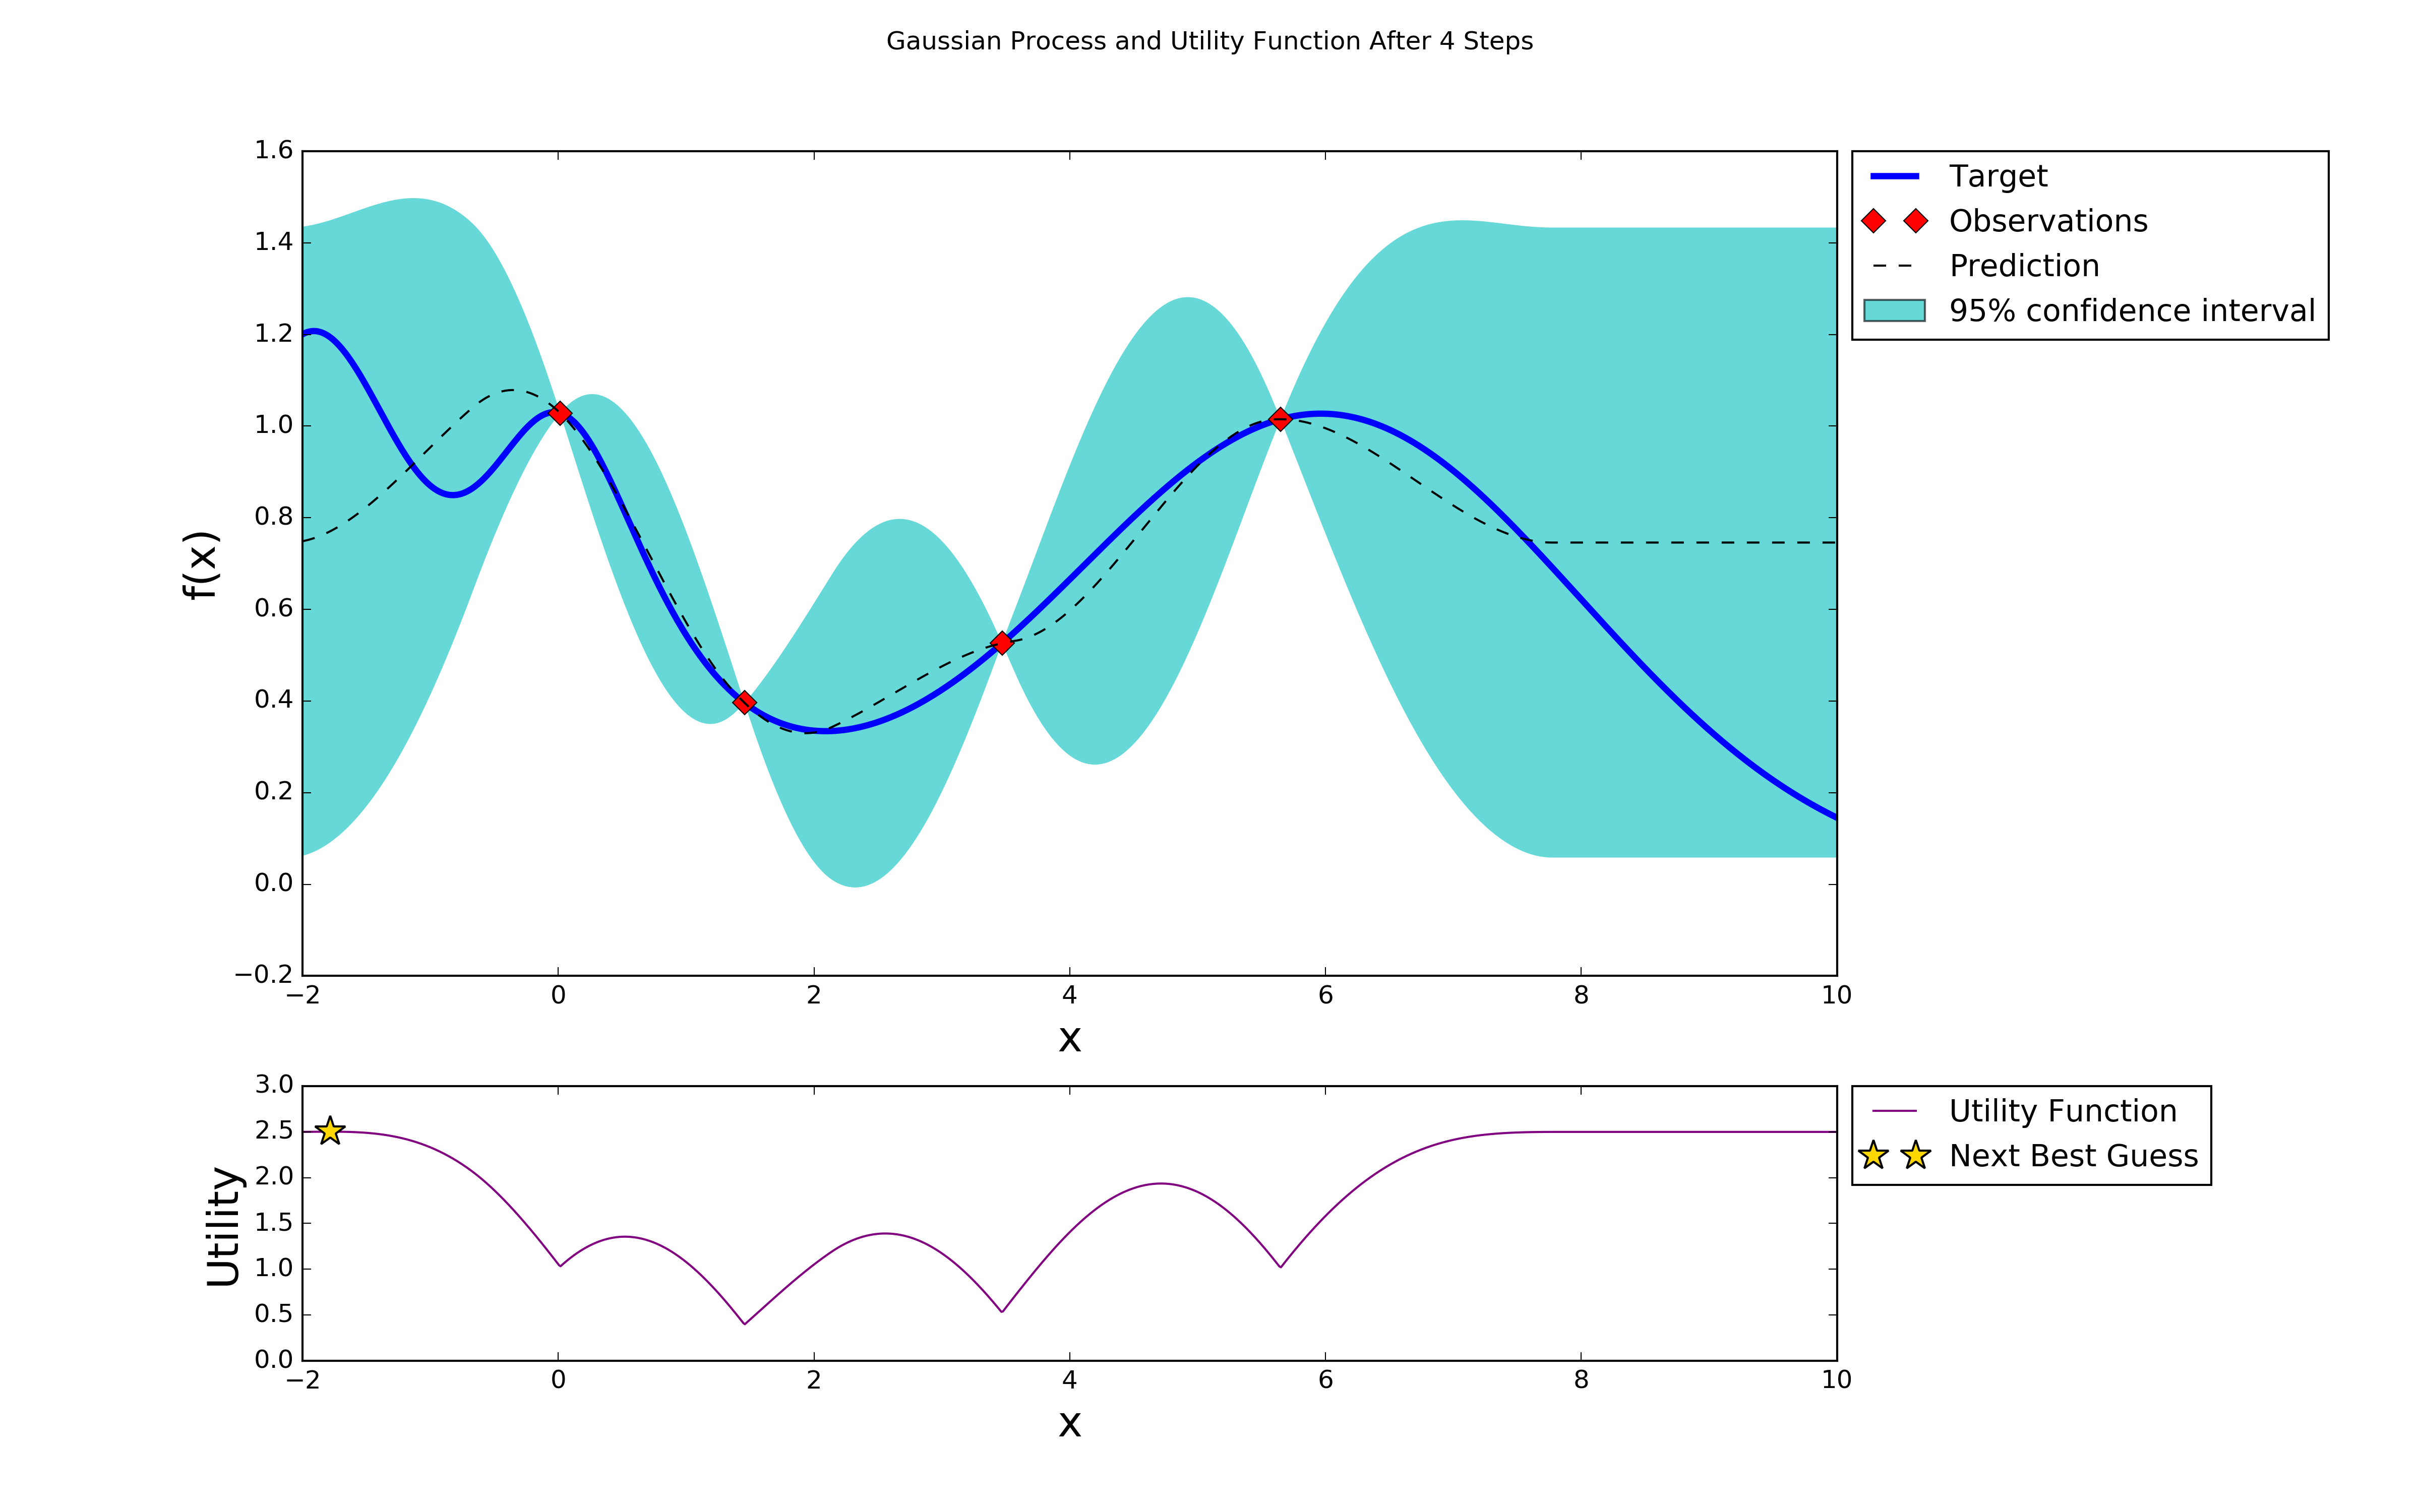
\includegraphics[width=1\textwidth]{figures/BO.png}
	\vspace{-2em}
	\caption{Example of an objective function and surrogate function. After probing observations from the objective functions the surrogate function is update to form the posterior. Uncertainty is low near observations.}
	\label{fig:bayesian-optimization}
\end{figure*}

\subsection{Kernel function}\label{sec:kernel-function}
The kernel is a function for the GP, which determines the smoothness of samples drawn from it. The choice of kernel is important in the process of fitting the Gaussian Process, to fit the objective function. Many kernels have been proposed, where one of the most used is the squared exponential function \citet{brochu2010tutorial}. The function however tends to smooth the surrogate function to much, to be applicable in real world problems. The kernel function used in this method will therefor be Matérn$\frac{5}{2}$, as proposed by \citet{snoek2012practical}.

\subsection{Acquisition function}\label{sec:acquisition-function}
When Bayesian optimization builds its model of the objective function, it iteratively choses inputs to sample outputs from the objective function. The choice of which inputs to sample from is determined by the \emph{acquisition function} (AF), which determines utility of sampling from a given input. Different acquisition functions yield different measures to make this decision. One measure is the \emph{Probability of Improvement} (PI) which given a candidate input computes the probability of improving the current best result. The probability of improvement at point $x$  can be computed with the Cumulative Distribution Function of the Probability Density Function of the random variable in the Gaussian Process at point $x$. 

Another approach is to consider the \emph{expected improvement} (EI) which not only takes into account the probability of improvement, but also the uncertainty, which is the variance of the Gaussian distribution of the surrogate at the given input. EI balances the trade-off between exploitation and exploring, and is therefore a well used acquisition function \citet{brochu2010tutorial}. $EI(x)$ is the function whch givs the expected improvement of choosing parameters $x$, and is defines as:
\begin{equation}
\label{eq:expected-improvement}
EI(x) =
\begin{cases}
   K + L & \text{ if } \sigma(x) > 0\\
   0 	  & \text{ if } \sigma(x) = 0
\end{cases}
\end{equation}
where $K = (\mu(x) - f(x^+))\Phi(Z)$ \\and $L = \sigma(x)\phi(Z)$ .
$\mu$ and $\sigma$ are the mean and variance of the posterior distribution of the surrogate function respectively, and $f(x^+)$ is the currently best result gained from probing the objective function. $Z$ is defined as:

\begin{equation}
\label{eq:expect-z}
Z =
\begin{cases}
\frac{\mu(x) - f(x^+)}{\sigma(x)} & \text{ if } \sigma(x) > 0\\
0 								  & \text{ if } \sigma(x) = 0
\end{cases}
\end{equation}
$\phi$ and $\Phi$ denote the \emph{probability density function} (PDF) and \emph{cumulative distribution function} (CDF) of the standard normal distribution.
The function for EI can then be used to probe the surrogate function with different parameter settings x, from where a new candidate point can be found to probe the objective function. The new candidate will be the parameter setting with the highest expected improvement.  

%- Combining posterior and refit the GP

\section{Random Forest Classification}

With the feature vector $\mathbf{X}$ extracted by the multi-class CSP algorithm as the training set, we train a classifier for multi-class motor imagery.

Several algorithms have seen popularity for classifying EEG data. The survey by \citet{chan2015systematic} on the performance of ensemble methods in EEG context argues that Random Forests more accurately classifies EEG data than other well-known methods such as k nearest neighbors and Support Vector Machines. \citet{sun2007experimental} also surveys the effectiveness of ensemble methods, but argues that performance is subject to the choice of base classifier as weak learners. To evaluate the results we train a Random Forrest classifier. We use the implementation from the Scikit-Learn library for Python \citep{scikit-learn}.   

The Random Forrest learning algorithm works by splitting the training set $T$ into $n$ subsets $\{t_1,…,t_n \quad | \quad t_i \subset S\}$ and trains $n$ decision trees for each subset $t_i$. The splitting is done randomly by drawing a \emph{bootstrap sample} with replacement e.g. sets are constructed by uniformly chosing samples, with the possibility that one sample is drawn more than once. When classifying new samples, the Random Forrest classifies on each of its decision trees and returns the mode result. Intuitively, the weak learners 'vote' on the result.

The decision trees are constructed by randomly splitting the training subset $t_i$ on the features to obtain the training subset $t’_i \subset t_i$ containing the feature values of the randomly chosen features, in the given subset. The decision tree is then constructed according to the C4.5 algorithm which constructs a node on the split with the highest information gain, and finally pruned for features which do not provide any improvements in model accuracy.

The hyperparameters in a Random Forest classifier is the number of weak learners used to build the classifier. Generally, the more weak learners used the better the model accuracy and for this reason we use one tree for each feature in our feature space given by the CSP algorithm. 

%------------------------------------------------

\section{Experimental Results}\label{sec:results}
In order to evaluate our method, we perform artifact correction and classification through the pipeline illustrated in \cref{fig:ProgramPipeline} on the BCI Competition IV dataset 2a \citep{brunner2008bci}. The dataset contains 4-class motor imagery EEG data from 9 subjects. Each subject participated in two sessions of 6 runs on different days. The training data is from the first session, and the test data is from the second. A run consist of 48 labeled trials, divided evenly between the 4 classes. Each trial measured the brain signals of a subject on 22 EEG channels and 3 EOG channels. We disregard the EOG channels since we are interested in correcting artifacts without any reference signals. Examples of trials, channels, runs, and sessions are shown in \cref{fig:dataset}. What we refer to as a trial is a three second span (750 samples) of motor imagery, i.e., without the cue, break, etc. in between.

\begin{figure*}
	\centering
	\begin{adjustbox}{width=\textwidth}
		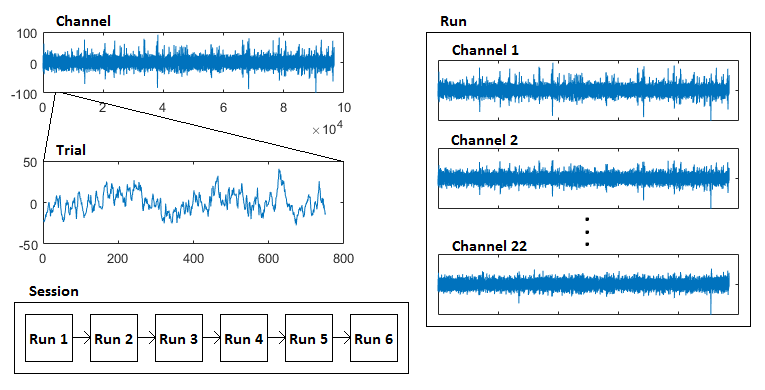
\includegraphics{figures/bciiv2a.png}
	\end{adjustbox}
	\caption{Sessions, runs, channels, trials, and the relations between them.}
	\label{fig:dataset}
\end{figure*}

We set up two pipelines to be compared. The first consists of artifact correction, followed by feature extraction with FBCSP and Random Forest classification. The second pipeline is identical but without the artifact correction step, i.e., just FBCSP and Random Forest. We run Random Forest with six predefined seeds and return the mean to ensure reproducibility.
To test the generality of the pipeline, we perform 6-fold cross-validation on the training data using five runs for training and one for validation. We run 200 iterations of Bayesian Optimization of select hyperparameters for each pipeline. The best hyperparameters from cross-validation for each pipeline is then used to construct the pipeline for the final evaluation, where we predict the labels for the test data. We repeat this for each subject. 
\cref{fig:results} shows the obtained accuracies with(C2) and without (C1) artifact correction for each subject.

\begin{table}[H]
	\begin{tabular}{@{}l|llll@{}} \toprule
		S					  & C1             & C2             & C3             & C4             \\ \midrule
		1                     & 83,04          & 82,29          & 81,42          & \textbf{83,85} \\
		2                     & 57,18          & 57,29          & 57,29          & \textbf{54,67} \\
		3                     & 78,18          & \textbf{79,16} & \textbf{79,16} & 75,64          \\
		4                     & 65,74          & 63,83          & 65,05          & \textbf{67,71} \\
		5                     & \textbf{58,85} & 55,21          & 55,21          & 56,94          \\
		6                     & \textbf{50,23} & 45,72          & 48,03          & 48,18          \\
		7                     & \textbf{68,75} & 68,69          & 68,69          & 67,94          \\
		8                     & 74,54          & 74,54          & \textbf{74,65} & 74,48          \\
		9                     & \textbf{75,64} & 72,97          & 72,80          & \textbf{75,64} \\ \bottomrule
	\end{tabular}
	\centering
	\caption{Accuracies for the best runs using 4 different setups. C1 is the baseline testing without OACL, C2 is 200 iterations of BO with OACL, C3 is 300 iterations of BO with OACL, C4 is 200 iterations with fixed parameters}
	\label{fig:results}
\end{table}

With 200 iterations the artifact correction did not overall yield better results than with no artifact correction and, in fact performed worse on some subjects. One possible cause may be that optimizing 27 parameters over 200 iterations is not a large enough budget to find optimal values for all hyperparameters, since the search space for 27 parameters is much larger than the search space for the 2 parameters optimized in the pipeline with no artifact correction. For this reason, we increased the iterations from 200 to 300 to see if this would yield improved results as illustrated in \cref{fig:i300}. As can be seen, the accuracy increased for three subjects, decreased for two, and remained the same for four. This indicates that 300 iterations are still not enough to optimize over such a large search space.


Because our objective is to determine whether removing the artifact signal from the raw signal yields improvements in classification accuracy, we manually set the non-artifact correction parameters to the best obtained values found in the non-correction evaluations, instead of further increasing the number of iterations. This introduces the assumption that good parameters without OACL are also good with OACL. Therefore, we now optimize the $\theta$ parameters to find the values that yield the highest accuracy. The results of running 200 iterations with this assumption are shown in \cref{fig:results}, as C4. \todo{discuss these results when we get them}

To determine the significance of these results we use the Wilcoxon signed-rank test. \Cref{fig:wilcoxon} shows the results of the test.



\subsection{Discussion}\label{sec:discussion}
% OACL ranges, may not only remove Ocular artifacts.
In the original OACL paper by \citep{li2015ocular}, the relative height ranges specified in \cref{eq:ranges} were determined by manual inspection of the characteristics of ocular artifacts. Since we generalized this as an optimization of hyperparameters, the found ranges are no longer guaranteed to be optimal in regards to ocular artifacts, but instead optimized for correcting the artifacts that most negatively affects the classification results. In fact, since we optimize the ranges for maximal classification accuracy, the method may be removing parts of the signal that are technically not artifacts, but removing them increases the performance of the classification model.

% Optimizing BO settings, and changing the kernel
Moreover, we have run Bayesian optimization with the default settings with regards to exploration vs. exploitation. Since running experiments on the pipeline with OACL is relatively expensive, it would be better to tune BO to spend more time on selecting the best candidate future sample to perform the next experiment on. The most used kernel for optimization problems used with BO is the squared exponential, this is however not always a good kernel, since sampling from a GP with this kernel, often will result in a unrealistic smooth function. Therefore we use Matérn 5/2 which is proposed in \citep{snoek2012practical}. Although this kernel function will be less smooth than the standard squared exponential, it might not be a suitable candidate for out optimization problem. In fact, BO might not even be possible with the domain of our parameters. BO assumes that input parameters with values close to each other, will have relatively similar outputs. Since our input space contains variables from many different algorithms, including FB, CSP and OACL, this assumption might however not hold. 

% Removing residual artifacts
As explained in \cite{hoffmann2008correction}, residual artifacts were still present after noise reduction methods were applied. We have also observed that residual artifacts are present, this can be seen in \cref{fig:oacl-signals}, where an event is registered around $x \approx 170$, but the following desynchronization/synchronization is not registered. A way that this could be handled is to always check if a residual artifact is present when an artifact is registered that, and mark it. These signals might need a separate $\theta$, since the signature of these artifacts is quite different from the artifacts introduced by eye blinks.

Since OACL is not restricted to finding ocular artifacts, a generalization of theta values for each channel, might not be optimal. This is due to the difference in how various artifacts shows in EEG data. A better way, might be to construct a classifier for artifacts, and use a different theta value for each such artifact. The classifier will then be used in the cleaning of new EEG signals, to remove just the right amount of artifact signal, based on the type of artifact. Furthermore, theta values are found based on optimization through BO. An alternative would be optimization through logistic regression. 
Since OACL is not restricted to finding ocular artifacts, a generalization of theta values for each channel, might not be optimal. This is due to the difference in how various artifacts shows in EEG data. A better way, might be to construct a classifier for artifacts, and use a different theta value for each such artifact. The classifier will then be used in the cleaning of new EEG signals, to remove just the right amount of artifact signal, based on the type of artifact. Furthermore, theta values are found based on optimization through BO.

An alternative would be optimization through logistic regression as proposed in the original OACL method by \citet{li2015ocular}. Even though their technique considered only binary classification, it would be possible to expand their logistic regression approach to the multi-class case, by applying an one-vs-rest algorithm to construct 4-binary classifiers. This should reduce the bayesian optimization search space, and increase the results of applying the ocular artifact correction.

% Using more oacl ranges
\todo{integrate the paragraphs below with discussion}
In this study we used just one range for OACL, but the method can easily be extended to use and optimize multiple ranges. That would likely increase the accuracy further, since different artifacts show up in different ranges. Each range adds to the dimensionality of the search space. Alternatively, a wavelet transform approach could be used for the removal step \citep{krishnaveni2006automatic}.

% More clever use of filter bank
The filter bank can be improved by optimizing over a wider variety of sub-bands, e.g., by mixing sub-bands with differing spans such as [4-8] and [8-11]. This would increase the complexity of the input space., which in turn would make the optimization of all parameters harder. 

%------------------------------------------------

\section{Conclusion}
The existence of artifacts is a persistent problem in EEG data that is detrimental to the efficacy of BCI systems. We considered the negative effect of ocular artifacts on motor imagery classification of 4-class EEG. As a possible solution to the problem, we presented a method for ocular artifact correction in multi class EEG data, as an extension to the binary class ocular artifact correction method OACL\citep{li2015ocular}. Furthermore, we showed that the hyperparameters that was manually determined in OACL, can be automatically tuned by application of Bayesian Optimization algorithm. By testing the ocular artifact correction on the BCI Competition dataset IV2a, we  we found that the best hyperparameters found after 200-300 iterations did not improve classification performance compared to classification without application of the ocular artifact correction method. We discuss that reasons for this include the problematically large optimization space over filtering parameters and that filtering parameters may not be generalizable over several trials.

Possible improvements for future work are adapting the logistic regression approach used by \citep{li2015ocular} for multi-class estimation of filtering parameters. Secondly, the detection and correction of the residual as a subprocess to the main artifact correction process. 
%Recapitulates the problem and the contribution.
%Assesses the significance of the contribution.
%Suggests and outlines future work, open problems, etc.

\section{Acknowledgement}
We thank Felipe Soares da Costa for valuable feedback. We would also like to thank Aalborg University for lending us hardware for testing program configurations.

%----------------------------------------------------------------------------------------
%	REFERENCE LIST
%----------------------------------------------------------------------------------------
\bibliographystyle{te}
\bibliography{references}

%----------------------------------------------------------------------------------------

\end{multicols}

\end{document}
